%%% SINGLE UPDATE FIGURES %%%

%% SINGLE UPDATE RELATIVE ERRORS %%
\begin{figure}[h]
    \centering
    \begin{subfigure}[b]{0.3\textwidth}
        \centering
        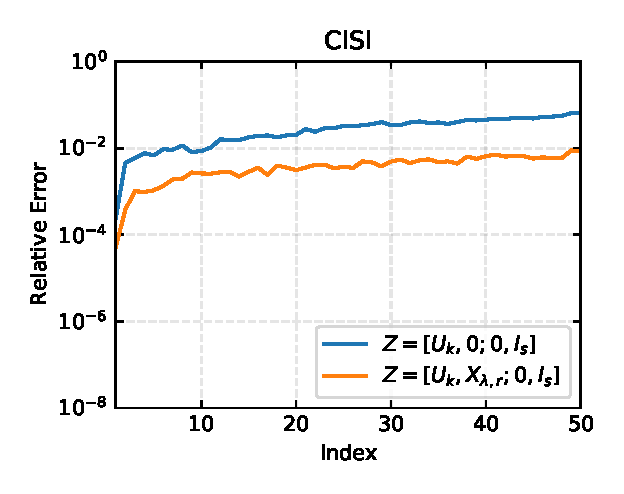
\includegraphics[width=\textwidth]{figures/single/cisi/relative_errors_CISI_batch_split_1.pdf}
        \caption{CISI}
        \label{fig:single_cisi_rel_err}
    \end{subfigure}
    %  \hfill
    \begin{subfigure}[b]{0.3\textwidth}
        \centering
        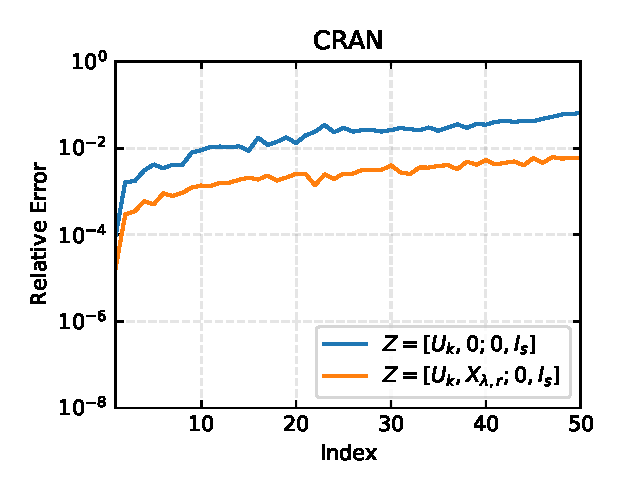
\includegraphics[width=\textwidth]{figures/single/cran/relative_errors_CRAN_batch_split_1.pdf}
        \caption{CRAN}
        \label{fig:single_cran_rel_err}
    \end{subfigure}
    %  \hfill
    \begin{subfigure}[b]{0.3\textwidth}
        \centering
        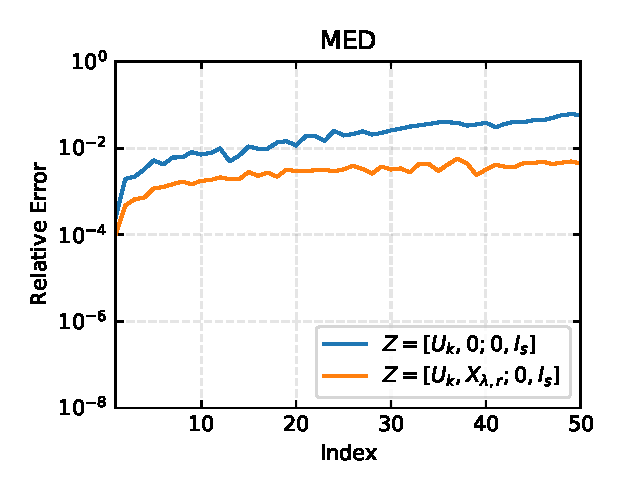
\includegraphics[width=\textwidth]{figures/single/med/relative_errors_MED_batch_split_1.pdf}
        \caption{MED}
        \label{fig:single_med_rel_err}
    \end{subfigure}
    %  \hfill
    \begin{subfigure}[b]{0.3\textwidth}
        \centering
        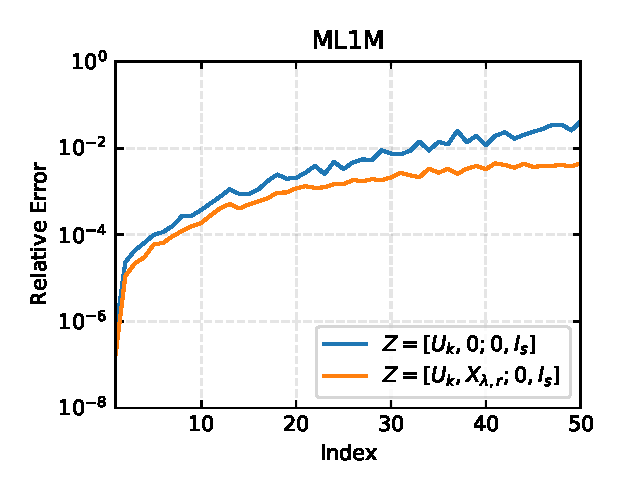
\includegraphics[width=\textwidth]{figures/single/ml1m/relative_errors_ML1M_batch_split_1.pdf}
        \caption{ML1M}
        \label{fig:single_ml1m_rel_err}
    \end{subfigure}
    %  \hfill
    \begin{subfigure}[b]{0.3\textwidth}
        \centering
        \includegraphics[width=\textwidth]{figures/single/reuters/relative_errors_reuters_batch_split_1.pdf}
        \caption{Reuters}
        \label{fig:single_reuters_rel_err}
    \end{subfigure}
    \caption{Relative approximation error of leading $k=50$ singular values in the single update case.}
    \label{fig:single_rel_err}
\end{figure}

%% SINGLE UPDATE RESIDUAL NORMS %%
\begin{figure}[h]
    \centering
    \begin{subfigure}[b]{0.3\textwidth}
        \centering
        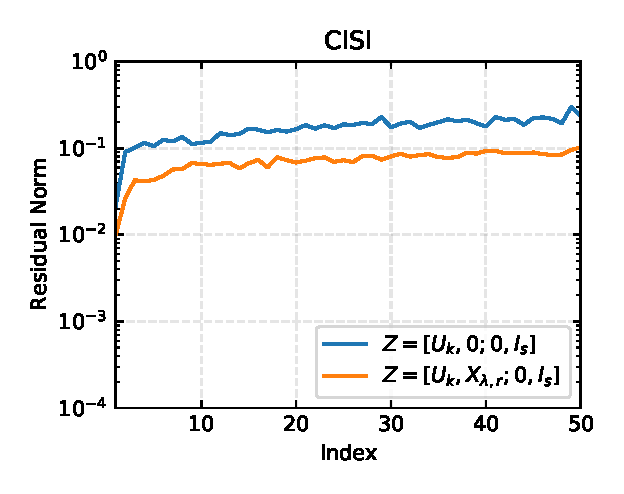
\includegraphics[width=\textwidth]{figures/single/cisi/residual_norms_CISI_batch_split_1.pdf}
        \caption{CISI}
        \label{fig:single_cisi_res_norm}
    \end{subfigure}
    %  \hfill
    \begin{subfigure}[b]{0.3\textwidth}
        \centering
        \includegraphics[width=\textwidth]{figures/single/cran/residual_norms_CRAN_batch_split_1.pdf}
        \caption{CRAN}
        \label{fig:single_cran_res_norm}
    \end{subfigure}
    %  \hfill
    \begin{subfigure}[b]{0.3\textwidth}
        \centering
        \includegraphics[width=\textwidth]{figures/single/med/residual_norms_MED_batch_split_1.pdf}
        \caption{MED}
        \label{fig:single_med_res_norm}
    \end{subfigure}
    %  \hfill
    \begin{subfigure}[b]{0.3\textwidth}
        \centering
        \includegraphics[width=\textwidth]{figures/single/ml1m/residual_norms_ML1M_batch_split_1.pdf}
        \caption{ML1M}
        \label{fig:single_ml1m_res_norm}
    \end{subfigure}
    %  \hfill
    \begin{subfigure}[b]{0.3\textwidth}
        \centering
        \includegraphics[width=\textwidth]{figures/single/reuters/residual_norms_reuters_batch_split_1.pdf}
        \caption{Reuters}
        \label{fig:single_reuters_res_norm}
    \end{subfigure}
    \caption{Norm of $A\hat{v}^{(i)} - \hat{\sigma}_i \hat{u}^{(i)}$ scaled by $\hat{\sigma}_i$ for leading $k=50$ singular triplets in the single update case.}
    \label{fig:single_res_norm}
\end{figure}